% Kolorowanie
\section{Kolorowanie}

\entry
Kolorowaniem (wierzchołkowym) grafu nieskierowanego nazywamy takie przypisanie kolorów
wierzchołkom grafu, że żadne dwa sąsiednie wierzchołki nie mają przypisanych tych samych kolorów.

\entry
Jeżeli istnieje kolorowanie grafu G z użyciem k kolorów, to mówimy że G jest k-kolorowalny.

\entry
Minimalną liczbę kolorów, którymi można pokolorować graf G nazywamy jego liczbą chromatyczną i
oznaczamy przez $\chi$  G 

\entry
Przez $\Delta $(G) oznaczamy maksymalny stopień wierzchołka w grafie G (stopień wierzchołka to liczba
jego sąsiadów w tym grafie)

\entry
Oczywiste: $\chi$ G ≤ $\Delta $(G) + 1.

\subsection{Brooks}

\entry
Każdy graf G różny od cyklu nieparzystej długości i grafu pełnego można pokolorować $\Delta $(G) kolorami.

\entry
Graf jest k-kolorowalny wtedy i tylko wtedy, gdy każda jego dwuspójna składowa jest k-kolorowalna.

\entry
Algorytm kolorowania Brooksa+ działa w czasie O(n+m)

\entry
Slajd:

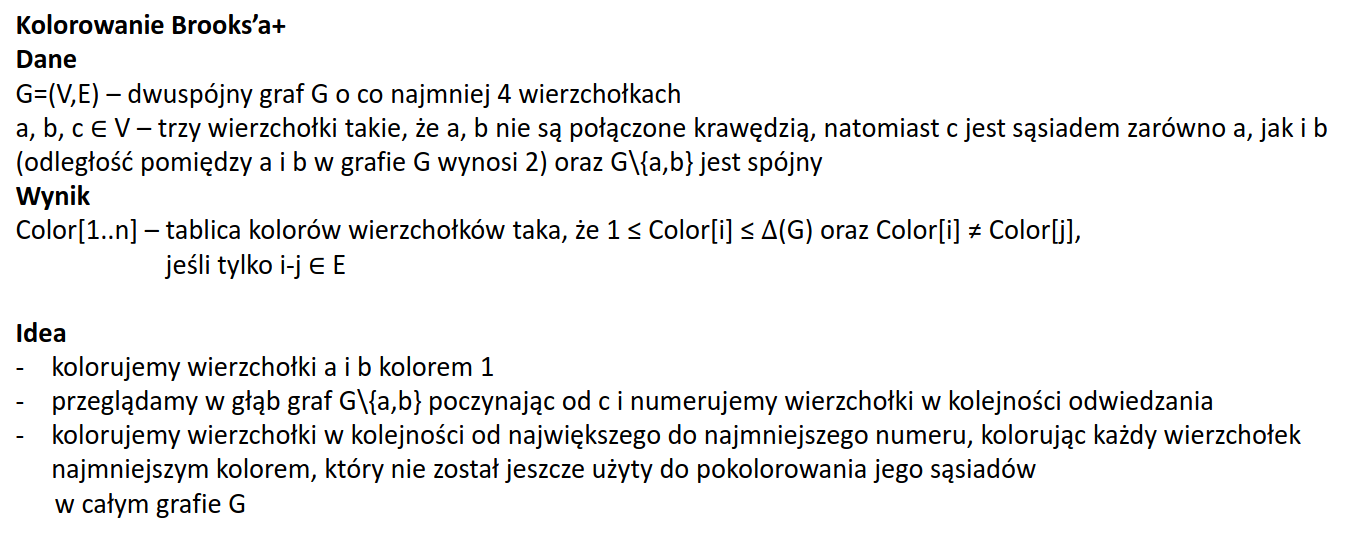
\includegraphics[scale=0.25]{boorks+.png}
